\capitolo{Rapporto di Trasmissione Ottimo}
Per ricavare il rapporto di trasmissione ottimo si utilizza una ottimizzazione a cui vanno associati ragionamenti aggiuntivi.

Nel caso di sistema motore + riduttore + carico vale la solita relazione \(C_m = (J_m+J_r)\frac{\AccAng_c}{\tau_r} + \tau_r \frac{T_2}{\eta_r}\), dove \((J_m+J_r)\frac{\AccAng_c}{\tau_r}\) è il contributo relativo l'albero veloce mentre \(\tau_r \frac{T_2}{\eta_r}\) è quello relativo l'albero lento.

\begin{figure}[h]
    \centering
    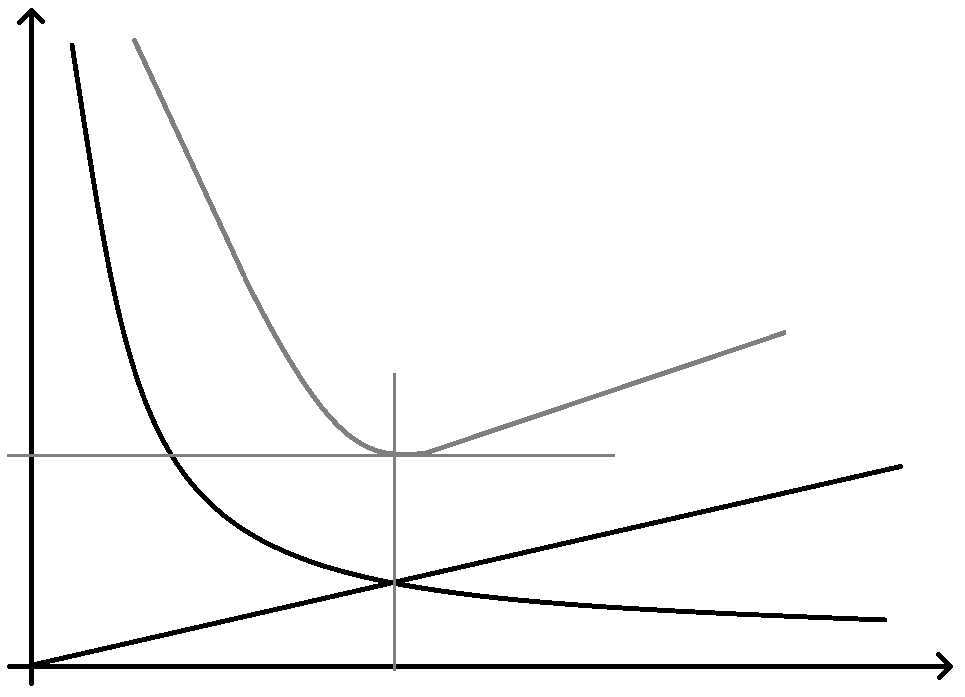
\includegraphics[width=0.4\textwidth]{Immagini/CoppiaTauRott.png}
    \caption{Rapporto di trasmissione ottimo}
\end{figure}


Per quell'espressione di coppia del motore è possibile ricavare il valore ottimo di rapporto di trasmissione \(\tau_{opt}\) di \(\tau_r\) tale che \(\minOtt{C_m}\), ossia \(\derivataparz{C_m}{\tau_r} = 0\), per cui vale:
\[ \tau_{opt} = \sqrt{\eta_r \frac{J_m + J_r}{T_2}\AccAng_c} \]
Per cui è importante notare che \(\eta_r, T_2, \AccAng_c\) sono tempo dipendenti, perciò anche il valore ottimo. In termini matematici ha senso, tuttavia per il progetto occorre avere un numero.
Delle grandezze temporali vanno considerati dei valori "medi" in particolare i valori RMS.

\sezione{Valutazioni sulla Coppia}
Parto dal considerare la coppia del motore RMS \(C_m^{RMS} = \sqrt{\frac{\int_0^{T_c} C_m^2(t)dt}{T_c}}\), scelta perchè minimizzare \(C_m\) significa minimizzare la taglia e quindi il costo di un motore.

\sottosezione{Caratteristica}
Dalla tipica caratteristica del motore PMSM (brushless) sono evidenti le zone di lavoro continuativo e intermittente.
Si può definire inoltre la \(T_{CS}\) ossia la Coppia Continuativa di Stallo (Torque Continuos Stall) punto per velocità nulla e coppia non nulla massima affinchè funzioni in regime continuativo. Inoltre la \(T_{CS}\) definisce la taglia del motore.

\(T_{CS}\) ha implicazioni per diversi parametri:
\begin{itemize}
    \item Massa cresce linearmente. In base alla famiglia, quindi alla tecnologia costruttiva, ci sono diverse curve.
    \item Costo cresce linearmente. In base alla famiglia, quindi alla tecnologia costruttiva, ci sono diverse curve.
    \item Inerzia cresce più che linearmente, quasi quadraticamente. In base alla geometria dell'albero quindi dal raggio e dalla lunghezza l'inerzia aumenta. La relazione è \(J_{cilindro} = \frac{1}{2} \rho L \pi R^4\)
    \item Attrito cresce linearmente\footnote{Guardare analisi di catalogo Parker.}
\end{itemize}

\sottosottosezione{Relazione Coppia di Stallo e Coppia RMS}
Nella fase di dimensionamento di un motore si devono unire la curva caratteristica del motore  e ciclo di riferimento, quindi verificare che il ciclo di lavoro sia composto da punti interni l'area di lavoro e che \(\left(C_m^{RMS},\VelAng_m^{RMS} \right)\) sia interno all'area di lavoro continuativa.
Quest'ultima si traduce in \(C_m^{RMS} < T_{CS}\) e quindi \(\minOtt{C_m^{RMS}}\) implica \(\minOtt{T_{CS}}\).

\begin{figure}[h]
    \centering
    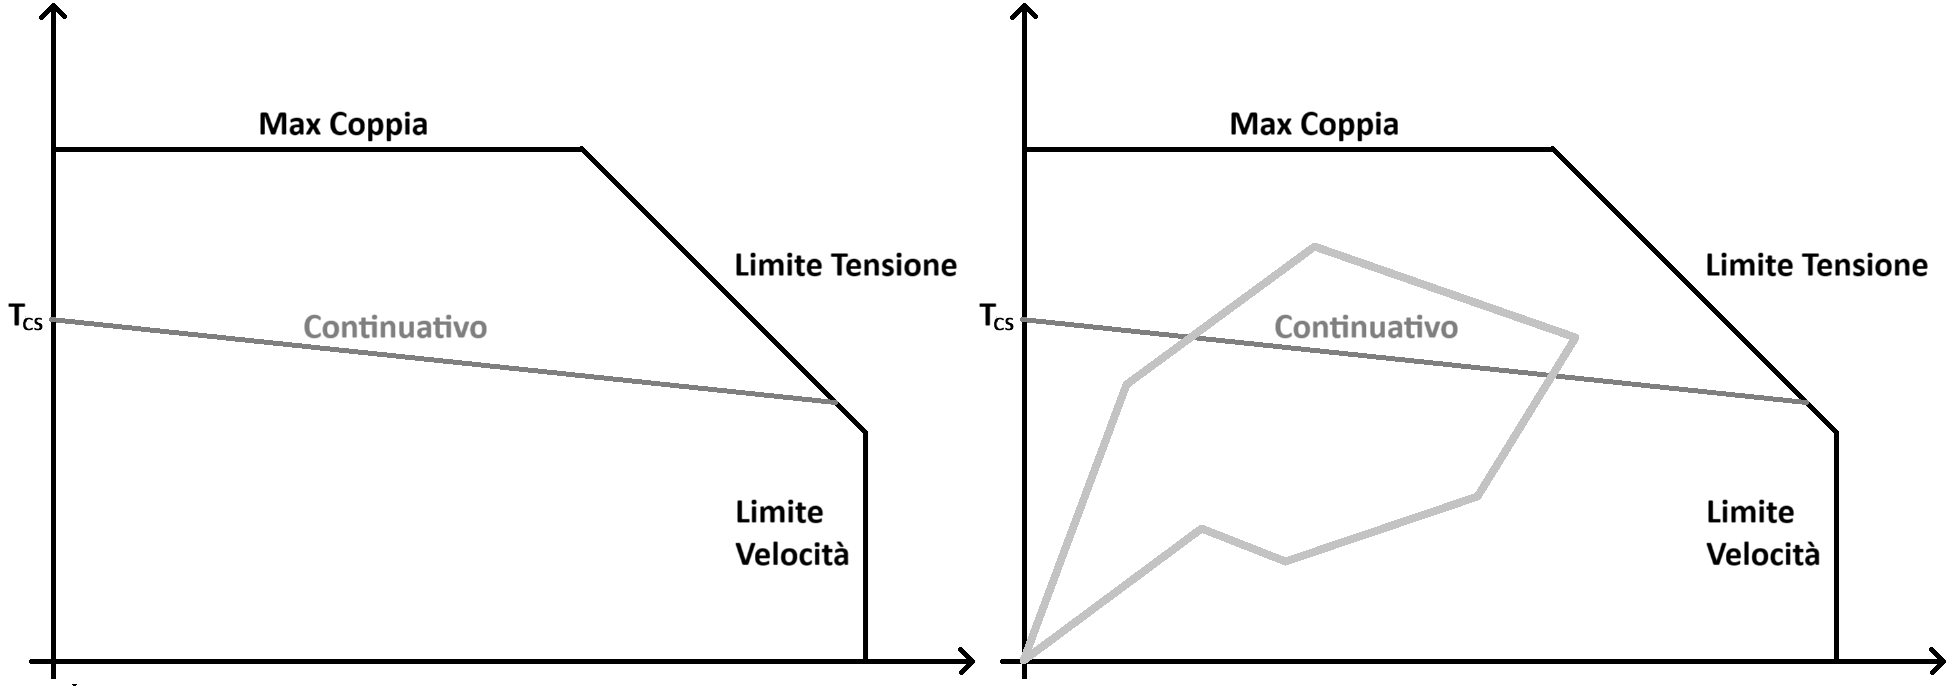
\includegraphics[width=0.6\textwidth]{Immagini/CaratteristicaPMSM.png}
    \caption{Caratteristica di PMSM con ciclo di lavoro}
\end{figure}

\sottosezione{Riformulazione con grandezze RMS}
Se si utilizzano le grandezze RMS la riformulazione risulta \(\tau_{opt} = \sqrt{\frac{J_m + J_r}{T_2^{RMS}/\eta_r^{RMS}}\AccAng_c^{RMS}}\). Considerando un rendimento alto, e che comunque il valore ottenuto dovrà essere adattato a quelli presenti nel catalogo disponibile, si può omettere il rendimento, si ottiene quindi un espressione indicativa per la scelta del \(\tau_r\):
\[\tau_{opt} = \sqrt{\frac{J_m + J_r}{T_2^{RMS}}\AccAng_c^{RMS}}\] 

\sottosezione{Vincoli}
Finora l'analisi non considerava i vincoli sulla scelta di rapporto di trasmissione.

\sottosottosezione{Rapporto di Tramsissione Minimo}
A limiti in termini di \(n_{1,max},n_{1N}\) si associa un vincolo di rapporto di trasmissione minimo \(\tau_{min}\), valori inferiori sono esclusi, questo potrebbe includere anche \(\tau_{ott}^l\), libero; in questo caso \(\tau^\text{vinc}_{ott} = \tau_{min}\) ossia il rapporto di trasmissione ottimo del sistema vincolato diventa il rapporto di trasmissione minimo\footnote{In modo simile a quanto visto per l'esercizio a pagina \pageref{EsercizioDimRid}.}.

\sottosottosezione{Rapporto di Trasmissione Massimo}
I vincoli di rapporto di trasmissione massimo sono legati a diversi aspetti.

\begin{enumerate}
    \item Risoluzione del trasduttore di posizione del motore riportato al carico, in particolare, detta \(\delta \theta_m\) risoluzione lato motore, \(\delta \theta_c = \delta \theta_m \tau_r\) ossia \(\tau_r\) piccolo permette di aumentare la risoluzione del carico, a discapito però di un calo della ripetibilità (precisione).
    \item Propagazione dell'errore di posizionamento del motore, in particolare detto \(\epsilon_m\) errore di posizione lato motore, riportato al carico diventa \(\epsilon_c=\epsilon_m \tau_r\), perciò migliora per \(\tau_r\) piccolo.
    \item Limite superiore al rapporto di inerzia \(\rho \) che è il rapporto tra la sommatoria dei momenti di inerzia lato carico riportati al motore su la sommatoria dei momenti di inerzia dell'albero motore. Nel caso in esame di motore riduttore e carico sarebbe\footnote{Nota bene che in realtà \(J_r\) andrebbe ripartita tra contributi di albero lento e albero veloce, tuttavia non sono noti.} \(\rho=\frac{J_c \tau_r^2}{J_m+J_r}\).
    Per \(\rho\) grande diventa più complicato il controllo del sistema in presenza di gioco o elasticità, viene quindi posto un \(\rho_{max}\) che si traduce in una limitazione del \(\tau_r\).
\end{enumerate}

In modo del tutto simile al caso di \(\tau_{min}\), anche il \(\tau_{max}\) potrebbe essere tanto stringente da escludere il valore \(\tau_{opt}^l\), libero, quindi  come prima se dovessere escluderlo occorre considerare un rapporto di trasmissione ottimo vincolato \(\tau_{opt}^v=\tau_{max}\).

\begin{figure}[h]
    \centering
    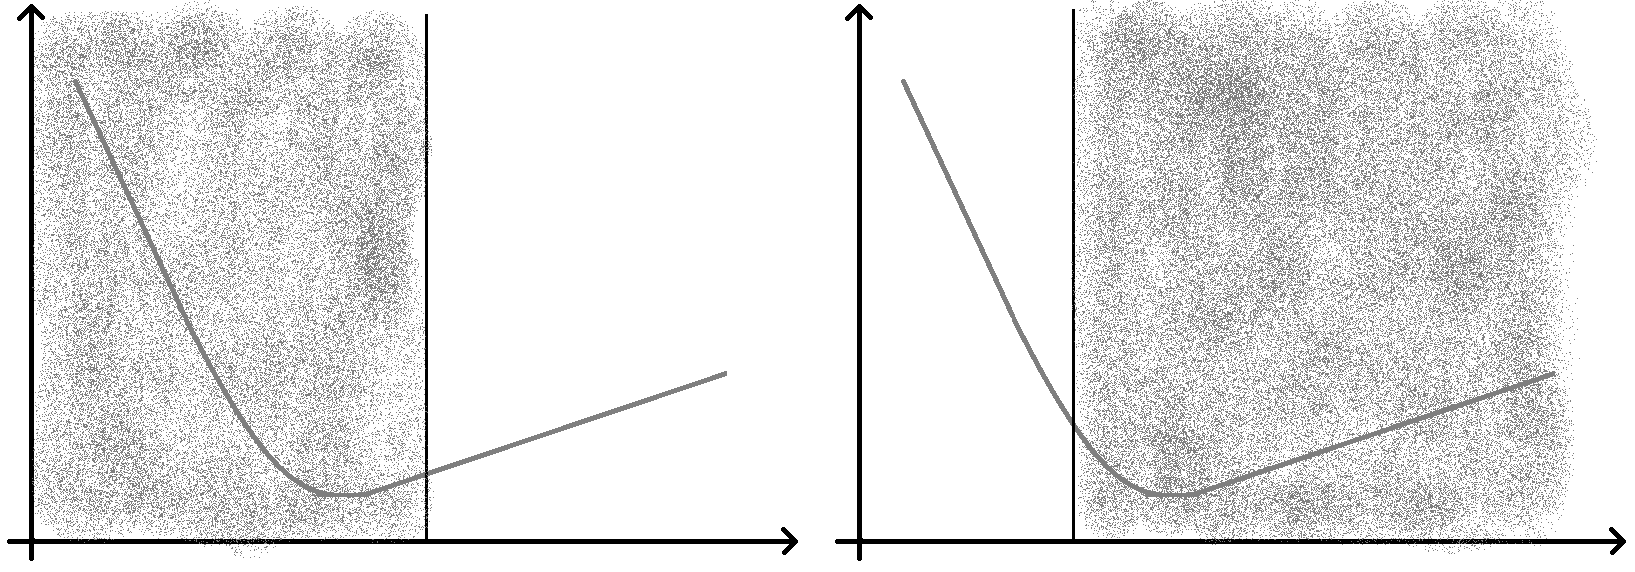
\includegraphics[width=0.6\textwidth]{Immagini/tauRmax_tauRmin.png}
    \caption{Rapporti di trasmissione: minimo sx, massimo dx}
\end{figure}

\sezione{Energia e Velocità}
Sono possibili altre valutazioni, in particolare un approccio che consideri l'energia elettrica assorbita e la velocità del motore.

\sottosezione{Energia Elettrica Assorbita}
L'energia elettrica assorbita è pari a \(E_m = \int^{T_c}_0 v(t) i(t) dt\),  considerando \(i(t)=\frac{C_m}{K_T}\) e \(v(t) = R i(t) + K_B \VelAng_m\), facendo opportune sostituzioni e manipolazione, si ottiene:
\[ E_m = \frac{R}{K_T^2} T_c (C^{RMS}_m)^2 + \frac{K_B}{K_T} \int^{T_c}_0 C_m\VelAng_m dt \]
Dove il primo dei due contributi tendenzialmente è dominante; occorre tuttavia tenere conto del secondo contributo che dipende dalla velocità e che quindi potrebbe diventare più rilevante.
Da queste valutazioni si trova che \(\minOtt{C_m^{RMS}}\) è simile a \(\minOtt{E_m}\), ma il rapporto di trasmissione ottimo per l'energia tendenzialmente è maggiore di quello per la coppia, perciò conviene utilizzare \(\tau_r >\) maggiori.

\sottosezione{Velocità del Motore}
La velocità del motore è inversamente proporzionale al rapporto di trasmissione, quindi per ottenere velocità inferiori conviene utilizzare \(\tau_r >\) maggiori.
Per velocità di motore elevate aumenta la coppia legata all'attrito viscoso; inoltre per velocità elevate \(K_T\) è ridotto, perciò la produzione di coppia richiede maggior corrente, quindi maggiori costi in termini di convertitori.